\chapter{Tests des Robotersystems}
\label{cha:Tests}

\section{Komponententests}

Das kontrollierte Testen eines Roboters ist nicht trivial. Aufgrund der Abhängigkeiten zwischen Hard- und Software reichen reine softwarebasierte Tests nicht aus. Bei der Übertragung der Befehle für Bewegung des Roboters  muss der Roboter tatsächlich vorhanden und betriebsbereit sein. Die Befehle müssen über eine bestehende Bluetooth-Verbindung an ihn übertragen und schließlich dessen Reaktion beobachtet werden. Daher wurde häufig auf die Methode des Ausprobierens (\enquote{Trial and Error}) zurückgegriffen. 

Komponenten wie die Objekterkennung wurden gesondert programmiert und manuell an realen Objekten getestet. Dies begann mit einfachen Versuchen in OpenCV. Erste Anwendungen waren das simple Erkennen der Farbe von Objekten. Anschließend wurden die besten gefundenen Parameter, wie beispielsweise  die Schwelle der Farbstärke des Erkennungsalgorithmus, ausgelesen und für den endgültigen Algorithmus verwendet. Auf diese Art wurde nach und nach um Objektverfolgung durch Kategorisierung und Erkennung der Form erweitert und die gut funktionierende Objekterkennung entwickelt wie sie nun in Betrieb ist.

Ein ähnliches Vorgehen wurde bei der Ansteuerung der Aktoren durchgeführt. Zunächst wurde der Grundaufbau des Roboters zum Testen mit einer im Play-Store erhältlichen allgemeinen Fernsteuerungs-App für NXT-Roboter \enquote{NXT Remote Control} \cite{nxt_remote_control} verwendet. Sie bietet nach Verbindungsaufnahme Bedienelemente zum Ansteuern jedes Motors an, was erste Fahrversuche des CLEEN-R-Roboters erlaubte. So wurde auch festgestellt, das der bestehende Aufbau die gestellten Anforderungen in Hinsicht auf Bewegungsfreiheit und Fähigkeit zur Objektaufnahme erfüllt und das Fahrgestell oder der Greifarm nicht weiter verändert werden müssen. Die Fernbedienungsapplikation erlaubte zusätzlich das Prüfen ob bei Ausfällen ein Hardwarefehler (Stromversorgung unzureichend, Bluetooth am NXT-Modul deaktiviert) oder ein Fehler in der Software (falsche Geschwindigkeit, abgebrochene Verbindung) vorlag. Dies erleichterte die Fehlersuche enorm.

Schließlich konnte so durch Ausprobieren, Optimieren und Erweitern unabhängig voneinander Steuerung und Objekterkennung nach und nach erarbeitet, letztendlich zusammengefügt und mit dem Roboter-Aufbau getestet werden.

\section{Manuelle Steuerung}

Zum Testen der Fahrfähigkeit, des Greifarms und der Positionsverfolgung wurde unter dem Einstellungsmenü der CLEEN-R App der Menüpunkt \enquote{manual control} hinzugefügt. Über ihn wird die in Bild \ref{fig:manualControl} gezeigte Activity gestartet, die dem Tester die Kontrolle über die Bewegungen des Roboters gibt.

\begin{figure}[h]
\centering
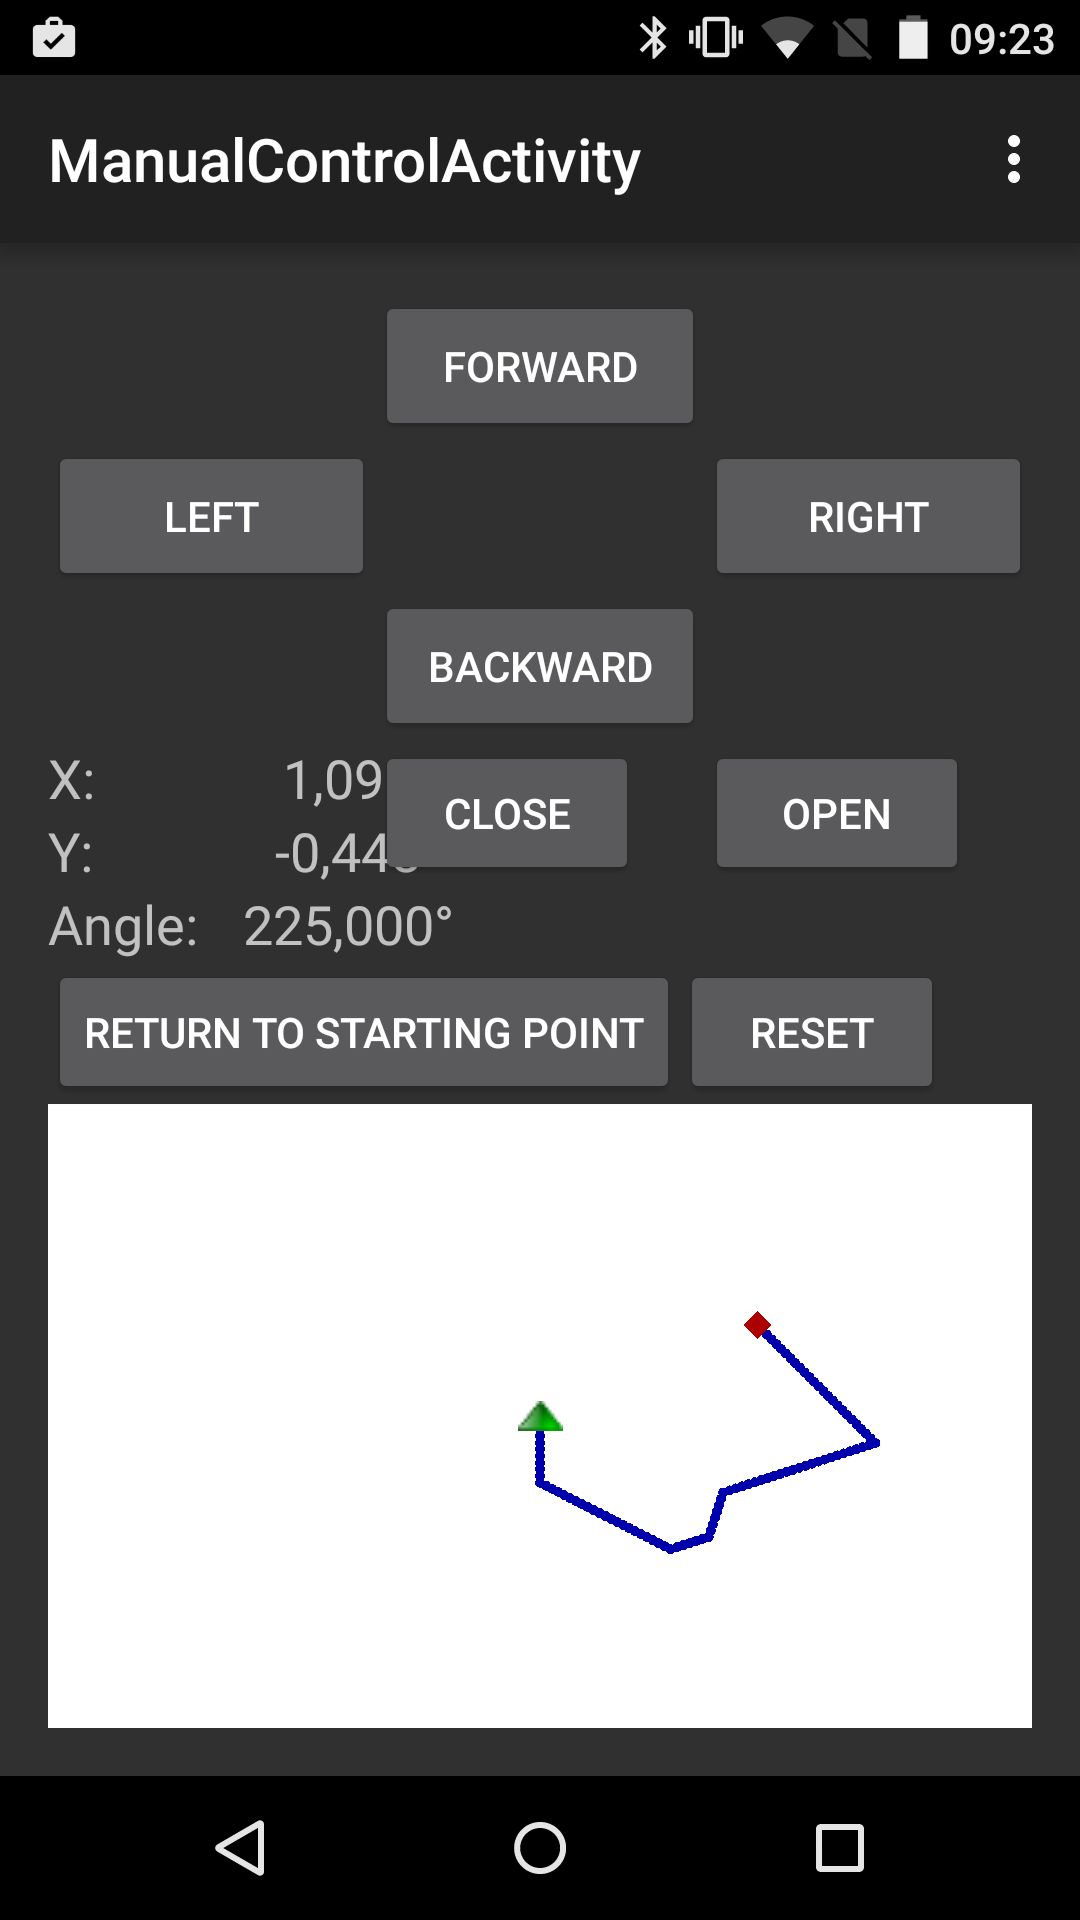
\includegraphics[width=0.4\textwidth]{Bilder/Tests/manualControl}
\caption{Manuelle Steuerung des Roboters}
\label{fig:manualControl}
\end{figure}

Das Smartphone wird für die direkte Kontrolle vom Roboter in die Hand genommen, die Übertragung der Befehle erfolgt wie im Normalbetrieb via Bluetooth. Über Buttons kann sowohl vor- und rückwärts gefahren, als auch im und gegen den Uhrzeigersinn rotiert werden. Des Weiteren lässt sich der Greifarm beliebig weit öffnen und schließen. Die aktuelle Position und der Winkel im Vergleich zum Start wird in Koordinatenform angezeigt und während der Bewegungen aktualisiert. 

Im unteren Teil des Bildschirms befindet sich eine graphische Repräsentation des Roboters und des bereits zurückgelegten Weges durch den Raum. Der Startpunkt wird ebenfalls markiert.

Nach dem manuellen Anfahren und Aufnehmen eines Objekts kann über den Knopf \enquote{Return to starting point} der Roboter wie in Kapitel \ref{sec:Rückkehr} vollautomatisch zum Startpunkt zurückgefahren werden. Über \enquote{Reset} wird die aktuelle Position des NXT-Roboters zurückgesetzt und als neuer Startpunkt festgelegt.

\section{Test des Gesamtsystems}

Ein Test des Gesamtsystems stellte sich als denkbar einfach heraus. Der Roboter wurde in einen weitgehend einfarbig weißen Raum platziert. Neben dem Robotersystem befanden sich zwei Gegenstände im Raum. Ein oranger Ball und ein blauer Würfel.

Der Roboter wurde über einen entfernten Laptop gestartet um nicht die Lichtverhältnisse des Systems zu beeinflussen und setzte sich nach wenigen Sekunden in Bewegung. Das System führte eine langsame Drehung um etwa 30\degree\ durch bis der etwa einen Meter entfernte blaue Würfel auf dem Display des Smartphones zu sehen war. Daraufhin rotierte das System etwas hin und her, bis der Würfel zentral auf dem Display und damit der Kameraaufnahme stand. Der Roboter bewegte sich einen halben Meter vorwärts, korrigierte die Ausrichtung nach und erreichte schließlich den Würfel. Der Greifarm griff etwas grob den Würfel, vollführte eine 180\degree\ Drehung und fuhr zum Startpunkt, der als Zielzone definiert war zurück. Bei der Rückfahrt musste der Roboter nicht korrigieren, verfehlte allerdings sein Ziel um etwa 12cm. 

Zu Beachten ist neben dem leichten Verfehlen der Zielzone, dass der Würfel nicht gehoben wurde, sondern auf dem Boden schliff. Dennoch erreichte der Roboter in unter einer Minute sein Ziel und begann mit der Suche des zweiten Objekts, welches auf Grund der fehlerhaften Position jedoch nicht in Reichweite der Kamera war und somit nicht gefunden werden konnte.

Es wurden zehn ähnliche Testläufe durchgeführt, von denen sieben wie oben beschrieben verliefen, zwei auf Grund von Softwarefehlern beendet wurden und einer bei dem beide Gegenstände die Zielzone erreichten.